% Latex template for MA305 Project Report, Spring 2015
%%%%%%%%%%%%%%%%%%%%%%%%%%%%%%%%%%%%%%%%%%%%%%%%%%%%%%%%%%%
\documentclass[11pt]{article}
\usepackage{graphicx}
\usepackage{color}
\newcommand{\cred} {\textcolor{red}}
\usepackage{fancyhdr}
\newcommand{\horrule}[1]{\rule{\linewidth}{#1}} 	% Horizontal rule

\begin{document}

%%%%%%%%%% TITLE PAGE %%%%%%%%%%
\begin{center}
{\it MA305, Spring 2017 \hfill Embry-Riddle Aeronautical University, FL 
 }
		\horrule{0.5pt} \\[0.4cm]
		{\bf \Large  Newton Iteration and Fractals}\\
		\horrule{2pt} \\[2cm]
%%%%%%%%%%%%%%%%%%%%
Kyle Latino \& Thomas Levine
\\[0.4cm]
23 April 2017 % change this
\end{center}

\begin{center}
\rotatebox{0}{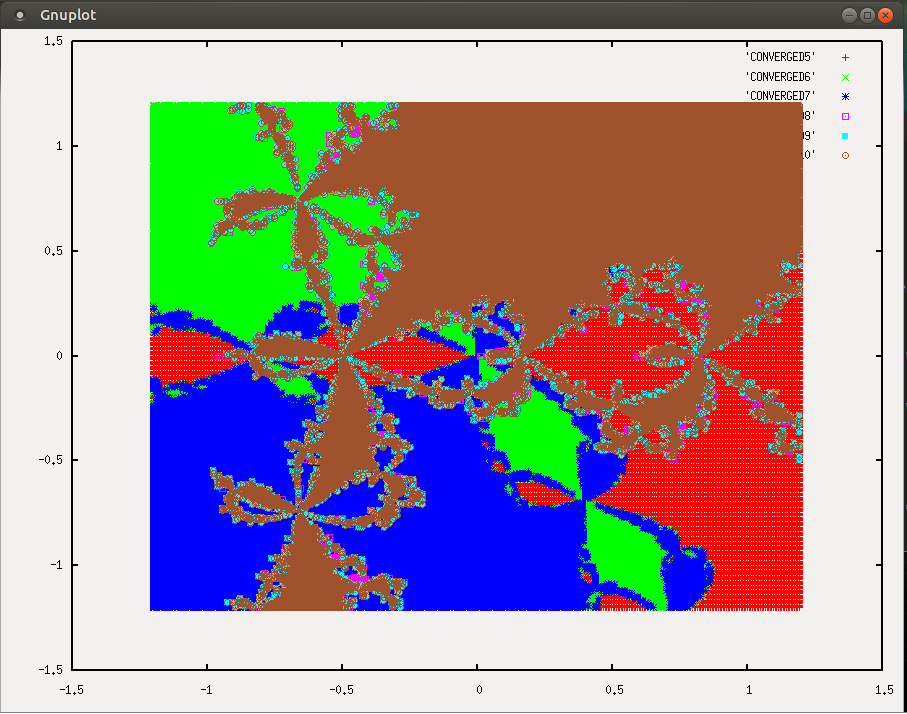
\includegraphics[scale=0.5]{everything.png} }
\end{center}

\thispagestyle{empty}
\newpage
\begin{abstract}

\end{abstract}
\tableofcontents 
\newpage

%%%%%%%%%%  %%%%%%%%%%
\section{Introduction}\label{S:1}
%The text of this section.
Fractals are interesting and arguably beautiful representations of repetition at varying scales. Some notable fractals are the Sierpinsky Triangle or the Menger Sponge. These figures have some interesting characteristics such as visibly repetitive patterns at any zoom and theoretically infinite surface area. The Menger Sponge can be found in modern wireless devices as its massive surface area allows it to be used as an antenna while maintaining a very compact size.


\section{Problem Statement and Assumptions}\label{S:2}
%The text of this section. 
This project is broken into two distinct parts. Part 1 requires that the Newton Method for root finding is implemented in Fortran. This is relatively simple as it only requires converting the method into an algorithm and transcribing the alogrithm to code. Part 2 in considerably more sophisticated. In part 2 we use the Newton Method to calculate points on a plane and tested the points for convergence. If they were found to converge, the points were written to a file and fed to gnuplot to display the resulting fractal.


\subsection{Newton Method for Root Finding}\label{S:2.1}
%Text introducing this subsection. 
In 1671 Sir Iaasic Newton developed a method for determining the roots of an equation. The pretense is: given an equation and an initial estimate for the root, you can iteratively approach the true root of the function. This method is superior to the simple bisection method in that it not only requires fewer input variables but also reaches the true value in fewer iterations. 

\subsection{Fractals from Newton Iterations}\label{S:2.2}
%Text introducing this subsection.
Using the Newton Method for root finding we will generate points and plot them using the open source tool gnuplot. To do this we set up a dat file named "fractal.dat" with the parameters this program to be "400 0.2 20 -1.2 1.2 -1.2 1.2" which are the values for M, R, N, A, B, C, and D respectively. We then wrote functions to calculate the value given a complex input for the given equation and its derivative in order to be able to compute the Escape-Time algorithm in order to complete the convergence tests. By running the Escape-Time algorithm for N iterations over an M+1 x M+1 matrix of complex numbers we were able to isolate the points that showed fractal structures along the ±60 and 180 degree rays for the first case. This convergence was determined by comparing the difference of the target function R. The target value was set to be one of each of the functions three roots, \[1+(0*i), .5+(sqrt(3)/2)*i, .5-(sqrt(3)/2)*i\] for the first equation \[(z^3) - 1\] and its derivative \[3*(z^2)\] in conjunction with the Escape-Time algorithm for Newton's iterations. \[z0 = z, zn+1 = zn − F(zn)/F0(zn), n = 0, · · · , Nmax.\] For the relaxed Newton method, \[z0 = z, zn+1 = zn − 2*F(zn)/F0(zn), n = 0, · · · , Nmax.\] the function, \[((z+1)^2)*((z^2)+0.25)\] its roots, \[-1+(0*i), -.5*i, .5+i\] and its derivative. \[(4*(z^3))+(6*(z^2))+(3*z)+0.5\] These different methods produced complex fractal patterns and were tested with varying input parameters. 



\section{Method/Analysis}\label{S:3}
%Text introducing this section
Begin with naming or characterizing the method/approach to be used, perhaps explain the basic idea behind it, to what type of problems it applies, under what conditions, what it achieves, what are its main features, advantages, disadvantages. Justify why it is applicable to this problem, stating clearly any assumptions you need to make about the problem for the method to apply. Name some other methods/approaches one could use, and if/why your method may be preferable.


\section{Solutions/Results}\label{S:4}
%Text introducing this section
Using a Ubuntu terminal we remotely connected to the WXSession server via a secure shell in order to gain access to the GNUplot tool.

\subsection{Newton Method}
%
The guess for the root of the function converges onto the true root within 6 iterations when using the Newton Method. Conversely, the bisection method requires 37 iterations to converge. This shows that for the function \[F(x)=x^3+x^2-3x-3\] the Newton method is able to find the root in 1/6th the time required by the bisection method.

Function roots: -1.7320508075688772, -1, 1.7320508075688774
\subsubsection{Newton's Cubit}
%
Newton famously used this method to solve only one function known as Newton's Cubit. \[F(x)=x^3-2x-5\]
Function root: 2.0945514815423265  

\section{Discussion/Conclusions}\label{S:5}
%Text introducing this subsection
We learned more about fractals, such as how they are developed over multiple iterations. The next project should have the 'chaos game' and/or 'Conway's game of life.' Or other fun computational problems that can take advantage of Monte Carlo Simulations.

\begin{thebibliography}{100}
\bibitem{a1}  
Dr. Khanal , Final Project assignment handout, 2017.
%
%\bibitem{a2}
%
%\bibitem{a3} 

\end{thebibliography}
\end{document}



%%%%%%%%%%%%%%%%%%%%%%%%%%%%%% section Appendix %%%%%%%%%%%%%%%%%%%%%
\appendix 
\setcounter{section}{0}           
\section{Codes and Makefiles}\label{S:A}
%
Text introducing the/this appendix.

Subsections and further divisions can also be used in appendices.

%%%%%%%%%% BIBLIOGRAPHY %%%%%%%%%%

\end{document}

\grid
